\chapter{Kravspecifikationer}
 Dette kapital omhandler en kravspecifikation som er blevet udarbejdet, udfra problemerne fra problemanalysen og idéer til projektetsløsning, som løsningen vil tage udgangspunkt i. Først vil en optimal løsning blive forklaret, hvilket er idéer uden nogen form for begrænsninger af tid, erfaring eller kunnen. Dernæst vil gruppens reele løsning være beskrevet, som så vil tage hensyn til de førnævnte begræsninger.

\section{Optimale løsningsforslag}
Den optimale løsning vil bestå af to dele, en mobiltelefon med GPS og en webservice som kan vise dataene sendt fra mobilen

Gruppen udarbejdede en række krav, som så blev sendt til Jens Børsting. Jens læste disse krav og funktioner igennem, kom med rettelser og tilføjelser, og på denne måde blev projektets krav og funktioner udarbejdet. 

Mobilen skal kunne:
\begin{itemize}
	\item Måle, sende og optage GPS positionen på løberen undervejs på ruten.
	\item Tilslutte sig en bestemt bane, som træneren har opsat og lagt på serveren inden træning.
	\item Mobilen må ikke hjælpe løberen undervejs i løbet, med at vise positionen på ruten.
\end{itemize}

Webservicen skal kunne:
\begin{itemize}
	\item Opsætte baner inden løbet.
	\item Være kompatibelt med GPS-ure.
	\item Vise løbernes position på kortet.
	\item Vise diverse statistik og data for løberens tur på banen. Dette vil være tider, afstande og hastigheder, samt en grafisk visning af den rute løberen har løbet.
	\item Sammenligne to løberes tur på samme rute, eller sammenligne med banens gennemsnit i forhold til statistik/rådata.
	\item Vise et grafisk replay af den rute løberen har løbet, med mulighed for at afspille flere løbere samtidig og dermed sammenligne vejvalg.
\end{itemize} 

Mobil-appen vil have en simpel brugergrænseflade hvor brugeren vil have mulighed for at vælge den bane vedkommende skal løbe. Herefter vil brugeren have mulighed for at trykke start, hvorefter mobilen kun vil vise hvor lang tid der er brugt indtil videre og en afslut knap. Under løbet sender mobilen løbende data om GPS position og tiden siden start. Når turen er løbet færdig trykker brugere på afslut og appen vil sende de sidste data og vise nogle resultater. Dette kan eksempelvis være tid i alt, højeste hastighed, gennemsnitshastighed, men også data om løberen sammenlignet med andre på samme bane. Dette kan f. eks. være hvor mange sekunder efter den hurtigste vedkommende har brugt på de enkelte stræk.

Inden løbet skal træneren eller arrangøren, kunne uploade den bane som personen har lavet, til serveren. Banerne kan vælges fra appen på mobilen, af de forskellige løbere. Efter løbet skal brugerne som sagt kunne uploade sine resultater til webservicen fra mobil appen, under og efter et endt løb. Disse resultater skal så kunne sammenlignes med de andre løbere, der har løbet den samme bane. Ud over at sammenligne statistik over løberens rute, som beskrevet ovenfor, skal den også kunne vise grafisk den rute som løberen har løbet. Derudover skal der være en replay funktion, så de vejvalg som løberen tager, kan ses. Så kan der indsættes flere løbere på den grafiske visning, så flere løberes vejvalg kan sammenlignes.

\subsection{Krav til optimalløsning}
Ud fra overstående har gruppen, i samarbejde med Jens Børsting, opstillet nogle krav til den optimaleløsning. Som udgangspunkt har gruppen gået ud fra at kravene skal være testbare. 

\begin{itemize}
\item Appen tilknyttet løsningen skal kunne køre på android smartphones og apple iphones.
\item Løsningen skal være en webservice.
\item Samme loginsystem for både app og webservice.
\item Webservicen skal kunne oprette og gemme baner i form af o-løbskort med integnede poster.
\item Webservicen skal grafisk kunne vise en eller flere GPS ruter uploaded fra appen ovenpå den tilknyttede bane (Kort)
\item Webservicen skal have følgende replay funktionaliteter:
\begin{itemize}
\item Det skal være muligt at til/fravælge løbere til den viste bane, evt. mulighed for at tilpasse halelængde (grafiske visning af løberens seneste antal punkter) og farve
\item Zoom funktion på kortet. (senere måske rotationsfunktion så kortet kan roteres og få strækretningen op på kortet.)
\item Det skal være muligt at starte og pause afpilningen af GPS Dataene.
\item Det skal være muligt at sætte tempoet til 1, 2, 5, 10 og 20 gange normal hastighed
\item Scrolling function for at komme hurtigt frem til et bestemt tidspunkt.
\item Det skal være muligt at vælge én post (punkt som alle passerer) hvor alle viste løbere bliver samlet ved. Der skal kunne defineres/vælges flere poster/punkter
\end{itemize}
\item Webservicen skal kunne vise følgende data for hvert stræk:
\begin{itemize}
\item Den enkelte løbers navn
\item Den enkelte løbers placering i løbet efter strækket
\item Den enkelte løbers stræk længde
\item Den enkelte løbers tilbagelagte rute
\item Den enkelte løbers samlede tid efter strækket
\item Den enkelte løbers tid på strækket
\item Den enkelte løbers tid i forhold til den hurtigste på strækket
\item Den enkelte løbers gns. fart på strækket
\item Den enkelte løbers top fart på strækket
\item Evt grafisk sammenligning mellem to løbere ved at tegne streger mellem de to løberes placering på samme tid efter udgangspunktet.
\end{itemize}
\item Appen skal kunne optage gps-data under løb og ved løbets afslutning sende disse til webservicen.
\item Appen skal kunne tilknytte sig en bane, oprettet på webservicen.
\item Appen skal kunne sortere banerne ud fra klub.
\item Appen må kun vise tid brugt hidtil og en afslutningsknap på skærmen under løbet.
\item Appen skal kunne tilgå og grafisk vise webservicens replayfunktionaliteter.
\item Appen skal være brugervenlig, i den forstand, at det skal være let at vælge en bane, starte et løb, afslutte et løb og bruge replay-funktionen. Navigering i appen skal være simpel.
\end{itemize}

\subsection{Mockup af optimalløsning}
\subsubsection{Mobilenhed}
Gruppen har gjort sig nogle tanker om hvordan den opmitaleløsning skal se ud og hvilke funktioner den skal have. Udfra dette er der blevet lavet nogle mugshots af hvordan gruppen tæntke den optimale løsning kunne komme til at se ud.

\begin{figure}
\centering
\begin{minipage}{.5\textwidth}
  \centering
  \fbox{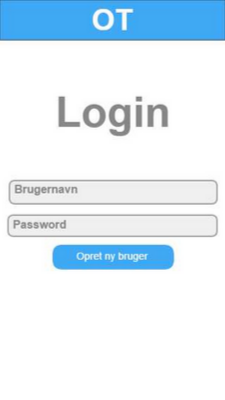
\includegraphics[width=.5\linewidth]{billeder/Mobilversion_1}}
  \caption{Login system}
  \label{fig:test1}
\end{minipage}%
\begin{minipage}{.5\textwidth}
  \centering
  \fbox{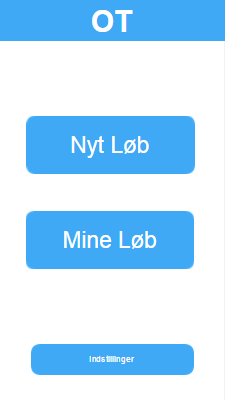
\includegraphics[width=.5\linewidth]{billeder/Mobilversion_2}}
  \caption{Mainmenu}
  \label{fig:test2}
\end{minipage}
\end{figure}

Figur 4.1 viser det første der ses når appen åbnes på ens smartphone. Der er to muligheder på denne side, enten kan der logges ind med en eksisterende bruger, eller også kan der oprettes en ny bruger. 
Hvis det lykkes at logge ind på appen, vil det næste der ses være figur 4.2, hvor der ses tre knapper. Der er mulighed for at påbegynde et nyt løb, der kan ses på de løb brugeren allerede har løbet, eller der kan ændres i ens indstillinger.

\begin{figure}
\centering
\begin{minipage}{.5\textwidth}
  \centering
  \fbox{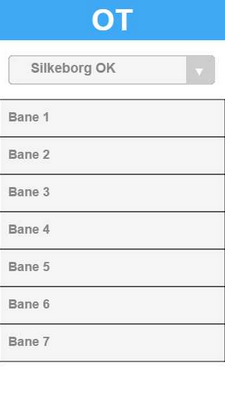
\includegraphics[width=.5\linewidth]{billeder/Mobilversion_3}}
  \caption{Menupunktet - Nyt løb}
  \label{fig:test1}
\end{minipage}%
\begin{minipage}{.5\textwidth}
  \centering
  \fbox{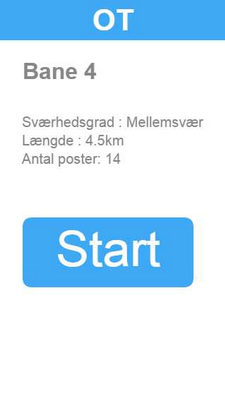
\includegraphics[width=.5\linewidth]{billeder/Mobilversion_4}}
  \caption{Informationer af valgte bane}
  \label{fig:test2}
\end{minipage}
\end{figure}
Hvis menu punktet ”Nyt løb” vælges, bliver brugeren ført videre til figur 4.3. Øverst i appen kan der ses en dropdown menu, hvor der er mulighed for at vælge den o-løbs forening som der løbes for. Under den valgte o-løbs forening, vil der så være et antal baner brugeren kan vælge at løbe. Det er foreningen selv der skal uploade de baner som er muligt at løbe, hvor det så er planen at en forening skal have et administrator login, for at kunne uploade disse baner.

\begin{figure}
\centering
\begin{minipage}{.5\textwidth}
  \centering
  \fbox{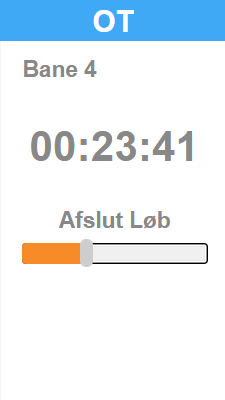
\includegraphics[width=.5\linewidth]{billeder/Mobilversion_5}}
  \caption{Appen underløbet}
  \label{fig:test1}
\end{minipage}%
\begin{minipage}{.5\textwidth}
  \centering
  \fbox{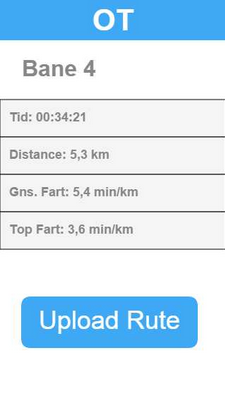
\includegraphics[width=.5\linewidth]{billeder/Mobilversion_6}}
  \caption{Appen ved afsluttet løb}
  \label{fig:test2}
\end{minipage}
\end{figure}

Trykkes der på en af banerne, eksempelvis bane 4.4, føres brugeren ind på siden set på figur 4.4. Her ses nogle informationer om det valgte løb, samt en stor ”Start” knap, hvor løbet selvfølgelig startes. De informationer der findes om løbet er sværhedsgraden på banen, ca. længden på banen, samt hvor mange poster løberen skal igennem. Hvis bane 4 er den bane brugeren gerne vil løbe, trykker brugeren på ”Start” knappen. Brugeren kommer så ind på en siden vist på figur 4.5. Denne figur afbilleder hvad der kan ses underløbet. Det er ikke muligt at se noget kort, da appen ikke skal vise løberens position på kortet. Det eneste der kan ses, er hvilken bane der er valgt, den tid der er gået siden der er trykket ”Start” og en slide knap til at afslutte løbet.
\begin{figure}
\centering
\begin{minipage}{.5\textwidth}
  \centering
  \fbox{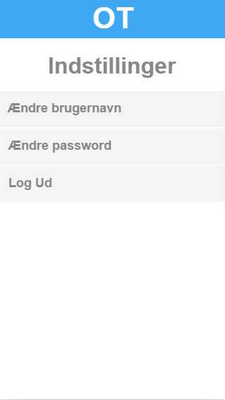
\includegraphics[width=.5\linewidth]{billeder/Mobilversion_7}}
  \caption{Menupunktet - Indstillinger}
  \label{fig:test1}
\end{minipage}%
\begin{minipage}{.5\textwidth}
  \centering
  \fbox{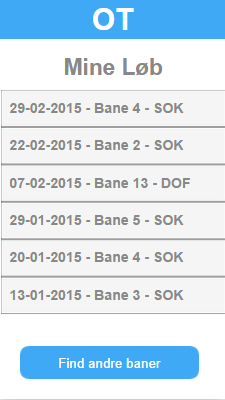
\includegraphics[width=.5\linewidth]{billeder/Mobilversion_8}}
  \caption{Menupunktet Mine løb}
  \label{fig:test2}
\end{minipage}
\end{figure}

Når løberen har været igennem alle poster og kommet i mål, bruges slide knappen ”Afslut løb”, dette fører brugeren ind på figur 4.6. Dette skal vise informationer om den netop færdiggjorte bane. Her ses tiden fra start til slut, den distance løberen har løbet, gennemsnitsfart og løberens top fart. I bunden af siden ses en ”Upload Rute” knap, trykkes der på denne knap uploades ens rute, over den bane der lige er blevet løbet, til webserveren. Nu kan løberens resultater sammenlignes med andre løberes resultater, på den specifikke bane.

Kigges der igen på figur 4.2 og menupunktet ”Indstillinger” vælges, bliver brugeren ført ind til figur 4.7. Her kan brugeren ændre sit brugernavn, sit password og vælge at logge ud fra appen.

Hvis menupunktet ”Mine løb” vælges i figur 4.2, kan brugeren se en liste over sine gennemførte løb, som ses på figur 4.8. Listen er sorteret efter dato, hvor de nyeste løb vil være øverst. Derudover kan der ses hvilken bane der er blevet løbet, samt hvilken forening der er blevet løbet ved. I bunden af siden er der en ”Find andre baner” knap, hvor der kan søges efter alle de baner der findes i databasen. Derudover kan der søges efter en specifik o-løbs forening eller dato, på denne måde kan der findes løb der er blevet løb på samme bane og dag som brugeren selv har løbet som ses på figur 4.9. De fundne baner kan så bruges til at sammenlignes med brugerens egne resultater på samme bane.

\begin{figure}
\centering
\begin{minipage}{.5\textwidth}
  \centering
  \fbox{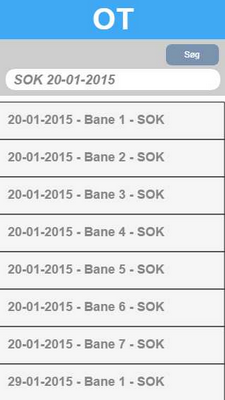
\includegraphics[width=.5\linewidth]{billeder/Mobilversion_9}}
  \caption{Find andre baner søge funktion}
  \label{fig:test1}
\end{minipage}%
\begin{minipage}{.5\textwidth}
  \centering
  \fbox{\includegraphics[width=.5\linewidth]{billeder/Mobilversion_10}}
  \caption{Evaluering- og sammenligningsværktøj}
  \label{fig:test2}
\end{minipage}
\end{figure}

Hvis brugeren har valgt at ville sammenligne løbere på en specifik bane, vil brugeren se en side lignende figur 4.10. I toppen af siden ses tre knapper. Den første er den side der allerede ses, hvor der er en grafisk visning af løberne på deres rute. Der ses en blå, rød og grøn slange på kortet, som er løberne. Under kortet findes der nogle mediaplayer funktioner. Den første knap er play/pause, den anden knap(flaget) bruges til at vælge hvilken post der ønskes sammenlignes fra. Normalt løber løberne ikke på samme tid, det ønskes dog lavet sådan, at det er muligt at sammenligne løbere fra en bestemt post. Dette betyder hvis løber 1 har en stræk tid på 2 min på post 1 og løber 2 har en stræk tid på 25 min på post 1, hvis løberne så ønskes sammenlignet fra post 1, ses der fra deres begyndelse fra post 1, lige gyldigt hvor lang tid de har brugt tidligere. De næste to knapper i mediaplayer funktionerne, bruges til at hoppe frem og tilbage mellem poster. Den sidste knap er en reset knap, hvor den fjerner alle de ændring brugeren har lavet tidligere, og sætter det op som det var i begyndelsen.  

Andet menupunkt i toppen, indeholder forskellige informationer om løberne. Dette er deres tider, distancer osv., så løberne også kan sammenlignes med tal og ikke kun grafisk. Sidste menupunkt er en guide der skal forklare hvordan dette sammenlignings værktøj bruges. Det skal forklare hvad de forskellige funktioner gør og hvordan de bruges.

Nederst på siden ses en knap ”Løbere”. Trykkes der på denne knap, skal et nyt vindue poppe op, hvor der skal være en liste over hvilke løbere der er med, og hvilken farve de har på kortet.
\subsubsection{Webservice}
Interfacet på webservicen ligner meget interfacet på appen fra figur 4.10. I toppen af figur 4.11 ser vi en hjemmeside title og menupunkter, som dog ikke krævere en større præsentation, da dette ikek vil indgå i det færdige produkt. I venstre side ses en anden menu, hvor første punkt er kortet som ses på billedet, andet punkt er en detaljeret statistik over løberne og sidste punkt er hjælpefunktion.
\begin{figure}[h]
    \centering
    \fbox{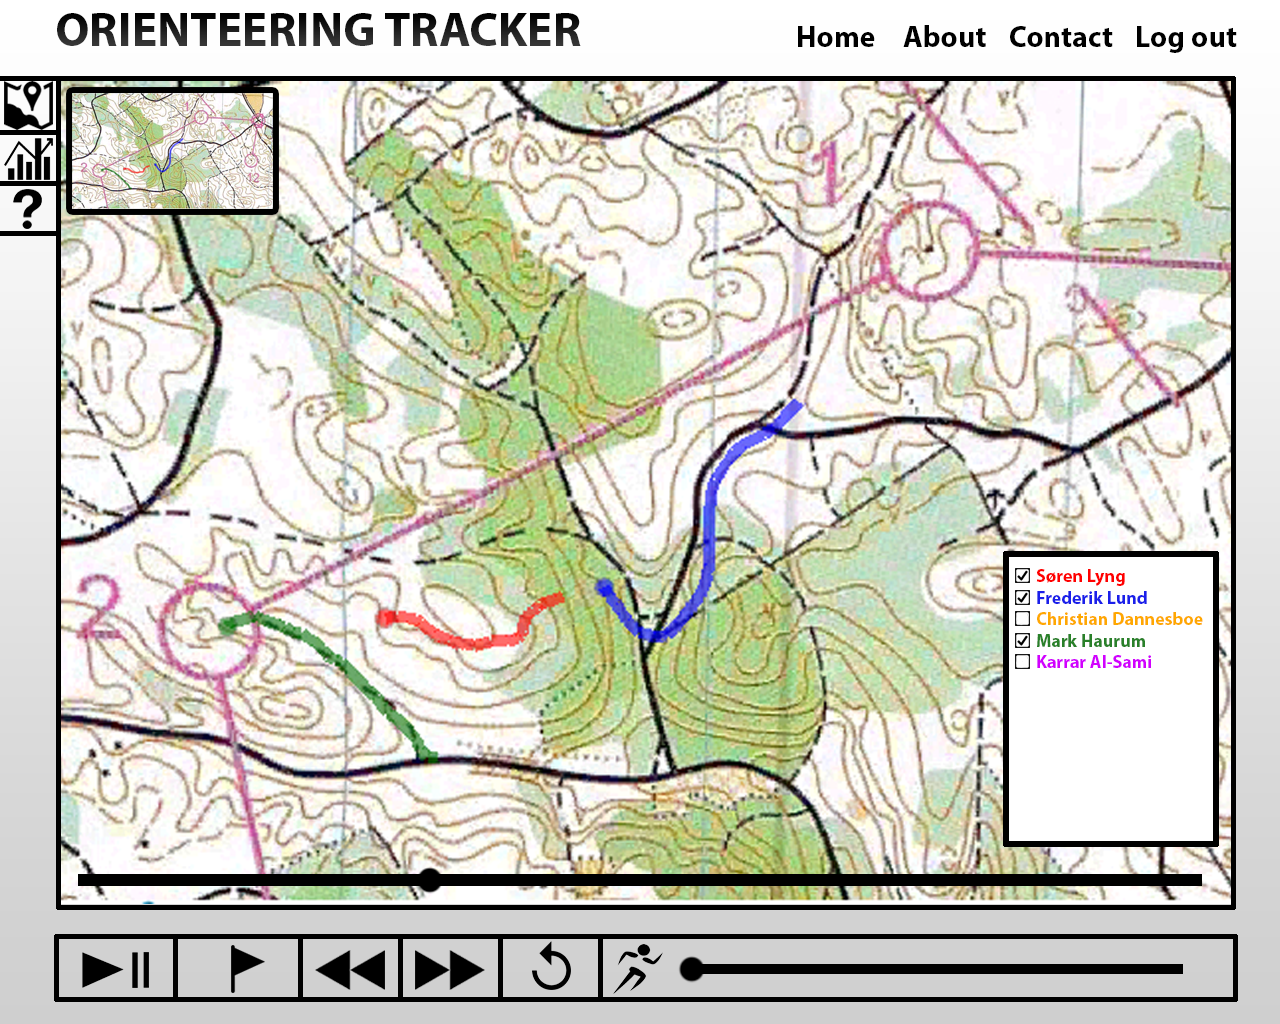
\includegraphics[width=.9\textwidth]{billeder/Website_udkast_1}}
    \caption{Interface til webservice}
\end{figure}

På figur 4.11 ses funktionen "Kort". Kort funktionen viser et orienteringskort, hvor løbernes rute kan genspilles. Øverst i venstrehjørne sidder et lille kort, der fungere som et oversigtskort. Oversigtskortet skal gøre det lettere at navigere rundt, da brugeren kan have en lettere forståelse af hvor de befinder sig på det store kort. Nede i højre hjørne findes en til og fravælgeses funktionen af de løbere, der er blevet tilvalgt til sammenligningen.

I bunden af figur 4.11 ses en mediaplayer. På denne findes der seks forskellige funktioner, hvor de her under vil blive beskrevet fra venstre mod højre: 
\begin{itemize}
\item Play/pause knap. Bruges som man kender det fra andre mediaplayere, til at starte og pause i sin afspilning.
\item Valg post funktion. Her kan der vælges mellem forskellige poster, hvorfra brugeren ønsker at se løberne løbe fra. Dette gør at løberne kan ses begynde fra samme post samtidigt, for bedre at kunne sammeligne deres vejvalg på deres stræk mellem posterne.
\item Forrige post. Sætter alle løbere til at løbe fra forrige post.
\item Næste post. Sætter alle løbere til at løbe fra næste post.
\item Refresh funktion. Fjerner alle indstillinger der er blevet tilføjet, og afspiller løbet som normalt.
\item Afspilningshastighed. Her kan afspilningshastigheden ændres.
\end{itemize}
Lige over mediaplayeren ses kan der ses hvor langt, brugeren er inde i genafspilningen af løbet. Den runde sorte plet, angiver hvor brugeren er nået til, hvor brugeren så også valgfrit kan springe rundt i genafspilningen.

\begin{figure}[h]
    \centering
    \fbox{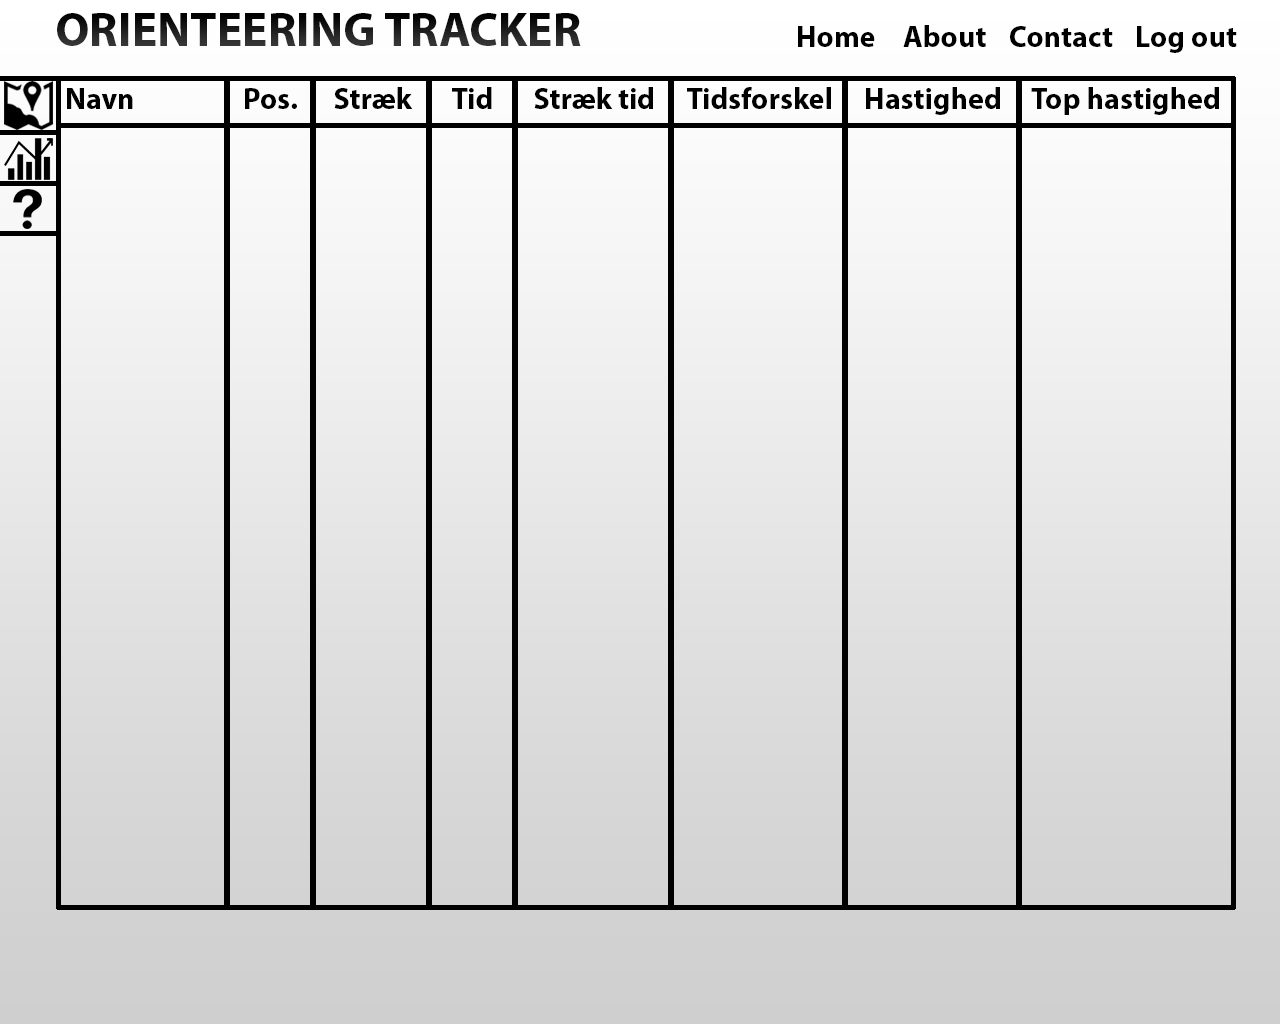
\includegraphics[width=.9\textwidth]{billeder/Website_udkast_2}}
    \caption{Detaljeret sammenligning af løbere}
\end{figure}

Figur 4.12 viser menu punktet om deltaljeret statistik over løberne. Under denne side kan der ses en række informationer om løberen under genafspilingen af løbet. Dette skal være en anden måde at sammenligne løberne, frem for kun at have den grafiske sammenligning. De ting der er tiltænkt, at skulle ses er løberens:
\begin{itemize}
\item Navn
\item Position i løbet
\item Hvor lang en distance de har tilbagelagt på det sidste gennemførte stræk
\item Tiden for løbet i alt
\item Tiden på det sidste gennemførte
\item Tidsforskellen mellem de forskellige placeringer, eksempelvis tidsforskellen mellem nummer et og nummer to i løbet
\item Gennemsnitshastighed
\item Tophastighed
\end{itemize}

Sidste menupunkt i venstre side er hjælpefunktionen. Meningen med denne funktion er, at den kunne hjælpe forvirrede brugere med brugen af programmet, hvis dette skulle blive en nødvendighed.

\section{Reelle løsning}
Ud fra listen over krav til den optimaleløsning i afsnit 4.1.1, har gruppen som at priortere hvad løsningen skal indeholde. Gruppen har ud fra den resterende tid og gruppens erfaring, valgt at priortere replayfunktionen med tilhørende kort højest. Selve projektet handler om at kunne sammenligne og evaluere en o-løbs træning, derfor er det vigtigt at kunne se de gode og dårlige beslutninger, en o-løber har taget på hans eller hendes rute. Som udgangspunkt vil der blive arbejdet på at kunne genspille en rute med én løber, derefter at kunne tilføje flere løbere, for at kunne lave ene sammenligning. Derudover har gruppen valgt at priotere den tekstbaserede sammenligning/statistik over løberne lige under replayfunktionen, som ses på figur 4.12. Dette gøres for at kunne give brugeren flere sammenlignings muligheder. Replayfunktionen giver et godt overblik over bl.a. vejvalg, men den teskbaserede sammenligning giver eksempelvis er mere detaljeret i forhold til hastighed, tid og distance.

Mobil-delen i projektet har gruppen valgt at simulere, hvor der optages GPS signaler på en smartphone, og filerne med længde- og breddegrader lægges over på computeren, og arbejdes med derfra. Samtidigt vil et kort anvendt i programmet kræve, at brugeren selv har et geostationært kort, dette vil blive nærmere forklaret senere i rapporten.

Nogle af punkterne i afsnit 4.1.1 kan ses nedenfor, hvilke er de punkter som gruppen har valgt at tageudgangspunkt i. Her ses de punkter der skal indgå i den grafiskvisning af løsningen:
\begin{itemize}
\item Det skal være muligt at til/fravælge løbere til den viste bane, evt. mulighed for at tilpasse halelængde og farve.
\item Zoom funktion på kortet.
\item Det skal være muligt at starte og pause afpilningen af GPS dataene.
\item Det skal være muligt at sætte tempoet til 1, 2, 5, 10 og 20 gange normal hastighed.
\item Scrolling function for at komme hurtigt frem til et bestemt tidspunkt.
\item Det skal være muligt at vælge én post (punkt som alle passerer) hvor alle viste løbere bliver samlet ved. Der skal kunne defineres/vælges flere poster/punkter.
\end{itemize}
Den tekstbaserede løsning skal kunne vise følgende den enkelte løbers:
\begin{itemize}
\item Navn.
\item Placering i løbet efter strækket.
\item Stræk længde.
\item Tilbagelagte rute.
\item Samlede tid efter strækket.
\item Tid på strækket.
\item Tid i forhold til den hurtigste på strækket.
\item Gns. fart på strækket.
\item Top fart på strækket.
\end{itemize}


\subsection{Brugervenlighed}
I gruppens problemformuleringen lød en af underpunkterne ” Hvordan kan løsningen gøres brugervenlig? ”. Gruppen har taget udgangspunkt i Rolf Molichs råd om brugrevenlighed, som har et speciale i software engineering: %http://www.dialogdesign.dk/Om_brugervenlighed.htm.

\begin{itemize}
	\item \textbf{Nyttigt} – Programmet skal løse de opgaver, som brugeren ønskes løst. 
	\item \textbf{Let at lære} – Programmet skal være let at lære at benytte, hvor indlæringstiden for at lære at løse bestemte opgaver skal være så kort som mulig.
	\item \textbf{Let at huske} – Her menes det at genindlæringstiden skal være så lav som muligt, for de brugere der har været væk fra programmet i en længere periode eller ikke bruger det så ofte. 
	\item \textbf{Effektivt at bruge} – Programmet skal køre og løse opgaver så hurtigt muligt. Der skal være så få fejl som muligt, hvis det skulle ske der forekommer en fejl, så skal kvaliteten af fejl meldingen være god.
	\item \textbf{Rart at bruge} – Dette er brugeren totaloplevelse af programmet, hvad deres mening er om det.
\end{itemize}

Rolf Molich nævner at alle disse egenskaber kan måles objektivt, hvor han giver eksempler som med et stopur eller spørgeskemaundersøgelser. Det program som gruppen har udviklet, er derfor prøvet at lave brugergrænsefladen så simpel og overskuelig som overhovedet mulig, samt løse opstående fejl. Da dette dog er det første store program som gruppen har lavet, har gruppen taget den beslutning at fokusere mere på at funktionerne i programmet til at virke, frem for at tænke på brugervenlighed.  Dette gøres pga. manglende erfaring med større programmer og den lille mængde tid der er til projektet. Brugervenlighed er dog stadig vigtigt i et godt program, så det vil gøres så simpelt som muligt. 

\subsection{Løsningsstrategi}
I dette afsnit vil planen for programmet blive beskrevet, med en overordnet beskrivelse af løsningsstrategi, samt en beskrivelse af valg mht. værktøjer brugt i udviklingen af programmet.

I henhold til gruppens kravspecifikation, vil GPS dataen til programmet blive simuleret af en app til en smartphone. Gruppen har brugt en app kaldet, myTracks til dette formål. myTracks optager og sender GPS signaler i form af en GPX-fil, som bliver tilsendt via e-mail til brugeren.
Som beskrevet i kravspecifikationen, skal brugeren sørge for at kortet anvendt skal være geostationært. Dette betyder, at der sammen med kortet medfølger en tekstfil med tal, der beskriver kortets placering på jordkloden. Med denne fil kan koordinater beskrevet med UTM-systemet (beskrives i teoriafsnittet), oversættes til pixels, og derved gøre det muligt at tegne afstandstro GPS-ruter på kortet. I dette projekt anvendte gruppen QLandkarteGT til at geostationære et kort, som blev anvendt til udvikling af programmet.

myTracks anvender koordinater i Lat/Long-formatet, hvor det geostationære kort oversætter UTM-koordinater til pixels. Dette betyder, at en konvertering fra Lat/Long til UTM er nødvendig, denne konvertering vil blive beskrevet i teoriafsnittet. 

Programmet vil her bestå af to dele, hvor den første del vil behandle data i form af pixels til at tegne ruter på kortet. Anden del af programmet vil bruge UTM-koordinater til at udregne data over løberne, som f.eks. hastighed og distance.

Til udviklingen af dette program har gruppen valgt at benytte Visual Studios Windows Forms, da gruppen ønsker at have en grafisk brugergrænseflade.